% ============================================================
% Training P&ID Digitizers Without Real Plant Data
% AI4RWC @ CVPR 2026 (Archival Track, 5-8 pages excl. refs)
%
% Build:  pdflatex main && bibtex main && pdflatex main && pdflatex main
%         or:  make  (see Makefile)
% ============================================================

\documentclass[10pt,twocolumn,letterpaper]{article}

% ---- CVPR 2026 style ----------------------------------------
\usepackage{cvpr}
\usepackage[pagebackref,breaklinks,colorlinks]{hyperref}

% ---- Standard packages --------------------------------------
\usepackage{times}
\usepackage{epsfig}
\usepackage{graphicx}
\usepackage{amsmath}
\usepackage{amssymb}
\usepackage{booktabs}         % \toprule, \midrule, \bottomrule
\usepackage{multirow}
\usepackage{makecell}         % \makecell for multi-line table headers
\usepackage{xcolor}
\usepackage{enumitem}         % tighter bullet lists
\usepackage[font=small,labelfont=bf]{caption}
\usepackage{microtype}        % better justification
\usepackage{siunitx}          % \pm alignment in tables
\usepackage{pgfplots}         % scale ablation figure (generated inline)
\pgfplotsset{compat=1.18}
\usepackage{tikz}
\usetikzlibrary{arrows.meta,positioning,shapes.geometric,fit,backgrounds,shadows}

% ---- Paper-specific macros ----------------------------------
% Dataset name macro — update before camera-ready if count changes
% Current corpus: 665 images (500 + 165 from two generation batches)
% Plan: generate to 1000 before submission; update \ours accordingly.
\newcommand{\ours}{SynthPID}
\newcommand{\method}{SynthPID}
% ± with small size in tables
\newcommand{\std}[1]{{\footnotesize$\!\pm\!$#1}}
% Bold result in table
\newcommand{\best}[1]{\textbf{#1}}
% Reviewer-safe anonymous citation placeholder
\newcommand{\anonrepo}{[anonymous repository, to be released upon acceptance]}

% ---- Colour scheme for qualitative figure -------------------
\definecolor{tp_green}{RGB}{34,139,34}
\definecolor{fp_orange}{RGB}{255,140,0}
\definecolor{fn_red}{RGB}{200,30,30}

% ---- CVPR review / camera-ready switch ----------------------
% Comment out the next line for camera-ready submission
\cvprfinalcopy

\def\cvprPaperID{****}
\def\httilde{\mbox{\tt\raisebox{-.5ex}{\symbol{126}}}}

% ============================================================
\begin{document}

\title{Training P\&ID Digitizers Without Real Plant Data}

\author{
    % Anonymised for double-blind review.
    % Camera-ready: replace with actual author list.
    Anonymous Author(s)\\
    {\tt\small anonymous@review.org}
}

\maketitle

% ---- Abstract -----------------------------------------------
% ============================================================
% Abstract
% ============================================================

\begin{abstract}
Digitizing Piping and Instrumentation Diagrams (P\&IDs) into structured
process graphs is critical for industrial operations, yet blocked by data
scarcity: companies cannot share proprietary plant drawings, and the only
public graph-annotated P\&ID benchmark contains just 12 real-world images.
Existing supervised methods require tens of annotated real P\&IDs for
training; synthetic alternatives fail because template-based generation
does not reflect real plant topology, yielding only ${\sim}33\%$ edge
detection accuracy.
We introduce \textbf{\ours{}}, a dataset of 665 topology-preserving
synthetic P\&IDs generated from 12 real-world seeds, and combine it with a
patch-based Relationformer pipeline adapted for high-resolution P\&IDs.
Training exclusively on \ours{} achieves \textbf{63.8\,$\pm$\,3.1\%
edge mAP} on PID2Graph~OPEN100 with no real training data --- 30~percentage
points above template-based synthetic, 18~points above the prior modular
baseline, and within 8~points of our real-data oracle.
A controlled comparison with~\cite{sturmer2025} (Appendix~A5) confirms
that the performance gap is attributable to generation quality rather than
model architecture.
A scaling analysis shows diminishing returns beyond 400 synthetic images,
implicating seed diversity as the primary constraint.
\ours{}, the generation pipeline, and trained models will be publicly
released upon acceptance.
\end{abstract}


% ---- Body ---------------------------------------------------
% ============================================================
% Section 1: Introduction
% ============================================================

\section{Introduction}
\label{sec:intro}

Real-world data is rarely accessible in safety-critical industries.
A single P\&ID digitization project at an industrial facility can require
months of expert annotation and significant cost — yet the resulting data
cannot be shared externally due to intellectual property constraints.
Piping and Instrumentation Diagrams (P\&IDs) are the primary engineering
document of process plants in the oil, gas, chemical, and power industries,
encoding every instrument, valve, pump, and pipe connection.
Maintaining a digital, queryable process graph from P\&IDs is critical for
safety audits, maintenance scheduling, and digital-twin
workflows~\cite{toghraei2019}.
Despite this industrial urgency, the only publicly available P\&ID dataset
with graph-level ground truth contains just 12 real-world images~\cite{sturmer2025}.

State-of-the-art end-to-end digitization requires tens of annotated real
P\&IDs for training.
Stürmer~\etal~\cite{sturmer2025} train on 60 real P\&IDs combined with
2,000 template-based synthetic images, achieving 75.46\% edge mAP on
OPEN100 --- but explicitly note that ``the Relationformer's performance
suffers significantly when trained on synthetic data only''
(Appendix~A5).
The standard response to data scarcity --- generate synthetic training
images --- does not resolve the problem when generation is template-based:
randomly placing symbols on a canvas yields graphs that do not reflect
industrial process topology, producing only ${\sim}33\%$ edge mAP on real
benchmarks~\cite{sturmer2025}.

We identify the root cause: the domain gap in P\&IDs is
\emph{structural}, not visual.
A model trained on synthetic graphs where components connect in random,
unrealistic topologies learns the wrong priors for real-world layouts.
Starting from just 12 real P\&IDs as seeds, our topology-preserving
generator creates \ours{} --- 665 training images whose graph statistics
mirror those of real industrial diagrams, with no additional annotation.
We pair this dataset with a patch-based inference strategy that processes
high-resolution P\&IDs at appropriate scale, following the approach of
\cite{sturmer2025} and adapting it for our synth-trained pipeline.

Training Relationformer exclusively on \ours{} achieves \textbf{63.8\%
edge mAP} on OPEN100 with \emph{zero real training data} --- 30
percentage points above template-based synthetic, 18 points above the
modular baseline that uses real data, and within 8 points of our
real-data oracle.
Adding even a small amount of real data (E3~Mixed) pushes to 72.6\% edge
mAP, approaching Stürmer~\etal's~\cite{sturmer2025} fully supervised result
of 75.46\% while requiring far fewer real P\&IDs.

This paper makes three contributions:

\begin{itemize}[noitemsep, topsep=3pt]
    \item \textbf{\ours{}}: the first topology-preserving synthetic P\&ID
          dataset with graph-level annotations, released with the
          generation pipeline and trained models upon acceptance.
    \item \textbf{Empirical evidence that generation quality is the
          bottleneck}: consistent with~\cite{sturmer2025} Appendix~A5,
          template-based synth achieves ${\sim}33\%$ edge mAP;
          our topology-preserving approach raises this to 63.8\%
          (+30~pp) using the same model.
    \item \textbf{A rigorous synthetic-to-real benchmark}: 5-fold
          cross-validation $\times$ 3~seeds on OPEN100 provides a
          reproducible evaluation framework for the data-scarce P\&ID
          digitization regime.
\end{itemize}

% ============================================================
% Section 2: Related Work
% ============================================================

\section{Related Work}
\label{sec:related}

\noindent\textbf{P\&ID Digitization.}
Early approaches decompose P\&ID digitization into sequential modules:
symbol detection using CNNs~\cite{rahul2019,mani2020,cha2019},
text recognition~\cite{baek2019craft}, and line detection via
Probabilistic Hough Transform~\cite{stuermer2023}.
These pipelines are brittle because errors in each stage propagate
forward, and the final graph is assembled without global structural context.
Jamieson~\etal~\cite{jamieson2024} survey the field and explicitly
identify data scarcity as the primary barrier to progress.
The first end-to-end graph-extraction approach is
Stürmer~\etal~\cite{sturmer2025}, who apply Relationformer to the
OPEN100 benchmark and achieve a 25\%+ improvement in edge detection over
the modular baseline.
Crucially, they require 60 annotated real P\&IDs for training.
We address the orthogonal question: what happens when none are available?

\noindent\textbf{Synthetic Data for Engineering Diagrams.}
Paliwal~\etal~\cite{paliwal2021} release Dataset-P\&ID, 500 synthetic
P\&IDs generated by randomly placing 32 symbol templates on a blank canvas.
Stürmer~\etal~\cite{sturmer2025} use a similar approach for pre-training
(2,000 template-synth images) but find that synth-only training
``suffers significantly'' on real diagrams (Appendix~A5).
Nurminen~\etal~\cite{nurminen2020} and Elyan~\etal~\cite{elyan2020} use
GAN-based augmentation for visual diversity, but GANs can only modify
image appearance — they cannot generate structurally new graphs.
We identify the root cause of the template failure: randomly placed symbols
produce graphs with unrealistic degree distributions inconsistent with
real plant topology.
Our topology-preserving generator addresses this directly.

\noindent\textbf{Simulation-to-Real Transfer.}
Domain adaptation from synthetic to real data is well-studied in
natural image settings~\cite{tobin2017,ganin2016}, but has received
little attention for structured diagram understanding.
The key insight from our work echoes findings in robotics sim-to-real
literature~\cite{akkaya2019}: structural fidelity of the simulated
environment matters more than visual realism for transfer.
For P\&IDs, \emph{graph topology} plays the role of physical dynamics —
a model trained on structurally unrealistic graphs fails to transfer
even when visual appearance is plausible.

\noindent\textbf{Image-to-Graph Transformers.}
Relationformer~\cite{shit2022} extends Deformable DETR~\cite{zhu2021}
with a shared relation token for joint object detection and edge
prediction.
EGTR~\cite{im2024} extracts scene graphs from DETR attention matrices
without bespoke relation tokens, achieving higher accuracy on Visual
Genome.
We adopt Relationformer following~\cite{sturmer2025} to ensure that
performance differences between our configurations are attributable to
training data rather than architecture.

% ============================================================
% Section 3: Method
% ============================================================

\section{Method}
\label{sec:method}

% ---------------------------------------------------------
\subsection{Task Definition}
\label{sec:method:task}
% ---------------------------------------------------------

Given a raster P\&ID image $I$, we aim to extract the process graph
$G = (V, E)$, where:
\begin{itemize}[noitemsep, topsep=2pt]
    \item $V$ is a set of detected physical components, each with a
          bounding box $(x_1, y_1, x_2, y_2)$ and a class label from
          \{\textit{valve, pump, instrumentation, general, tank, arrow,
          inlet/outlet}\};
    \item $E$ is a set of pipe or signal connections between components,
          each labelled \textit{solid} or \textit{non-solid}.
\end{itemize}

\noindent\textbf{Connector collapsing.}
\label{sec:method:collapse}
Raw P\&ID annotations contain \textit{connector} nodes
(${\approx}8\times8$~px routing waypoints) and \textit{crossing} nodes
(pipe-over-pipe non-connections) that together account for 50--65\% of
all annotated nodes but carry no physical meaning.
We collapse connector chains into direct component-to-component edges
(majority-vote edge label along each chain) and remove crossing nodes
before training and evaluation.
This reduces the problem to industrially meaningful connectivity and
aligns with the evaluation protocol of~\cite{sturmer2025}.

% ---------------------------------------------------------
\subsection{Topology-Preserving Synthetic Generation}
\label{sec:method:generation}
% ---------------------------------------------------------

\begin{figure*}[t]
    \centering
    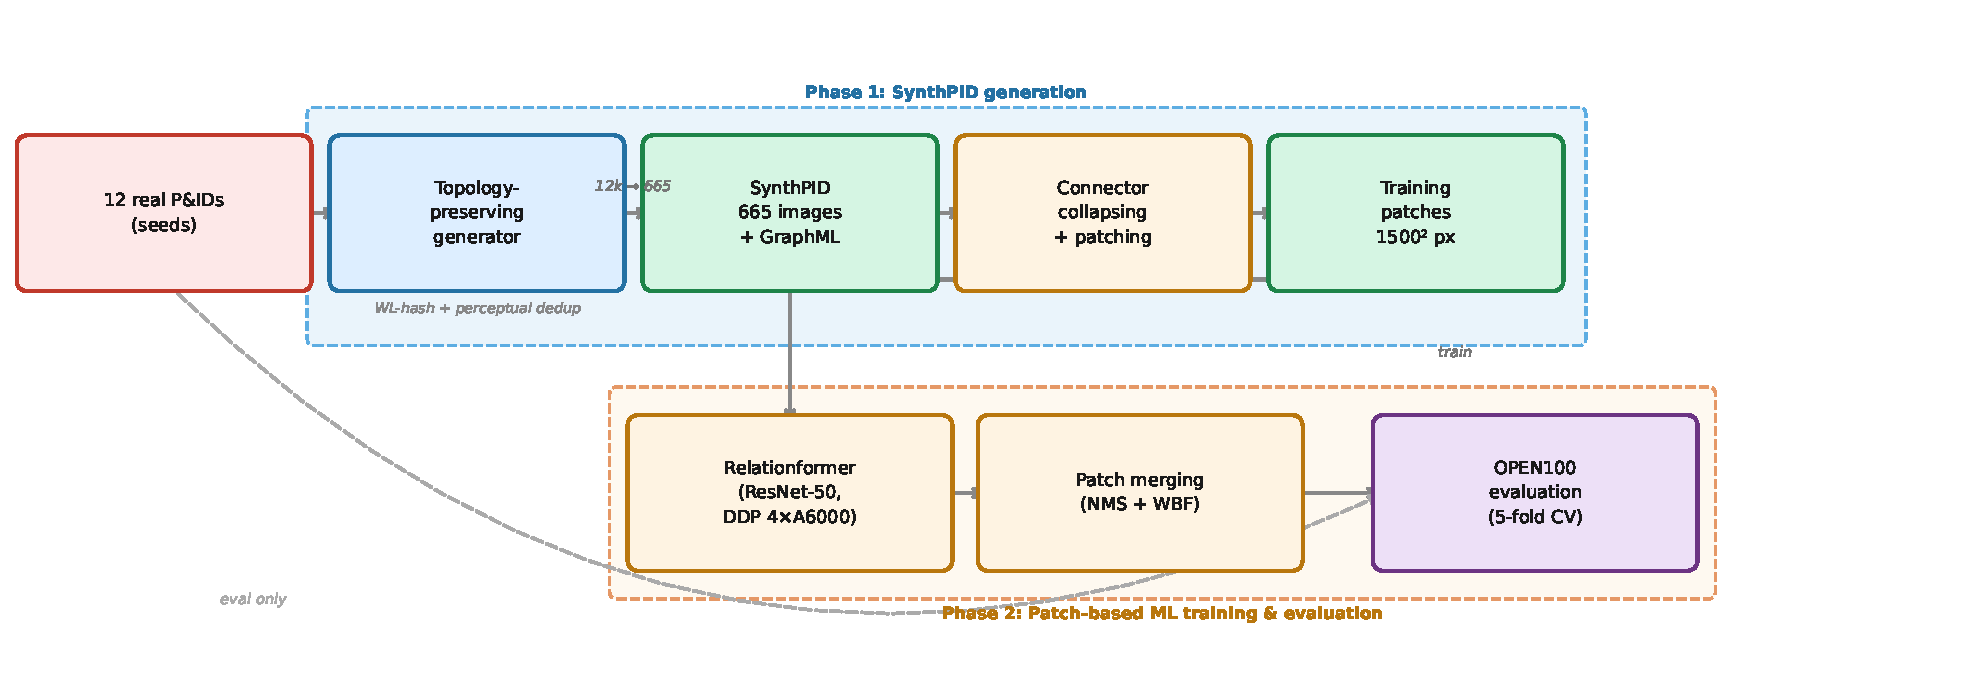
\includegraphics[width=\linewidth]{figures/pipeline_overview.pdf}
    \caption{
        \textbf{Overview of our approach.}
        Starting from 12 real-world P\&ID seeds, our topology-preserving
        generator produces \ours{} --- 665 structurally diverse
        synthetic P\&IDs with full graph-level annotations.
        A Relationformer trained on \ours{} with no real training data
        processes each P\&ID via overlapping patches and merges the
        resulting predictions into a complete process graph, which is
        evaluated on unseen real OPEN100 P\&IDs.
    }
    \label{fig:pipeline}
\end{figure*}

Figure~\ref{fig:pipeline} illustrates the full pipeline.
The key departure from prior work is \emph{how} synthetic data is created.

\noindent\textbf{Template-based generation (prior work).}
Existing synthetic P\&ID datasets~\cite{paliwal2021,sturmer2025} place
symbol templates at random positions on a blank canvas and connect them
according to a simplified grid layout.
The resulting graphs have unrealistic degree distributions and spatial
structure inconsistent with real process plants.
This mismatch explains the poor transfer reported
in~\cite{sturmer2025} (${\sim}33\%$ edge mAP with synth-only training).

\noindent\textbf{Topology-preserving generation (ours).}
We seed the generator from real P\&IDs.
Each generation step proceeds as follows:
\begin{enumerate}[noitemsep, topsep=2pt, leftmargin=1.3em]
    \item \textbf{Seed extraction.} Apply connector collapsing to a real
          P\&ID to obtain the physical component graph
          $G_s = (V_s, E_s)$.
    \item \textbf{Structural perturbation.} Spatially perturb node
          positions within topological constraints; substitute symbols
          within the same class for visual diversity.
    \item \textbf{Edge routing.} Re-route pipe connections via
          Manhattan routing while preserving graph adjacency.
    \item \textbf{Rendering.} Render the perturbed layout to PNG
          alongside a synchronised GraphML annotation.
    \item \textbf{Quality control.}
          Reject the candidate if its Weisfeiler-Lehman
          hash~\cite{shervashidze2011} matches any previously accepted
          graph (structural deduplication), or if its perceptual
          hash~\cite{phash} matches any prior image (visual
          deduplication).
\end{enumerate}

From ${\sim}12{,}000$ generation attempts seeded from 12 real P\&IDs,
we accept \textbf{665 structurally and visually diverse} synthetic
P\&IDs, constituting \ours{}.

\noindent\textbf{Visual and structural domain gap.}
Figure~\ref{fig:dataset_comparison} illustrates the visual gap between
real and synthetic P\&IDs: real OPEN100 diagrams have white backgrounds,
black line art, and professional title blocks, while SynthPID images have
a grey background and slightly different rendering style.
Despite this visual gap, the two corpora share the same symbol vocabulary
and, crucially, realistic pipe topology — which Figure~\ref{fig:graph_stats}
confirms quantitatively.
Our main result (63.8\% edge mAP) demonstrates that topology alignment
is sufficient for effective synthetic-to-real transfer even in the
presence of this visual gap.

\begin{figure}[h]
    \centering
    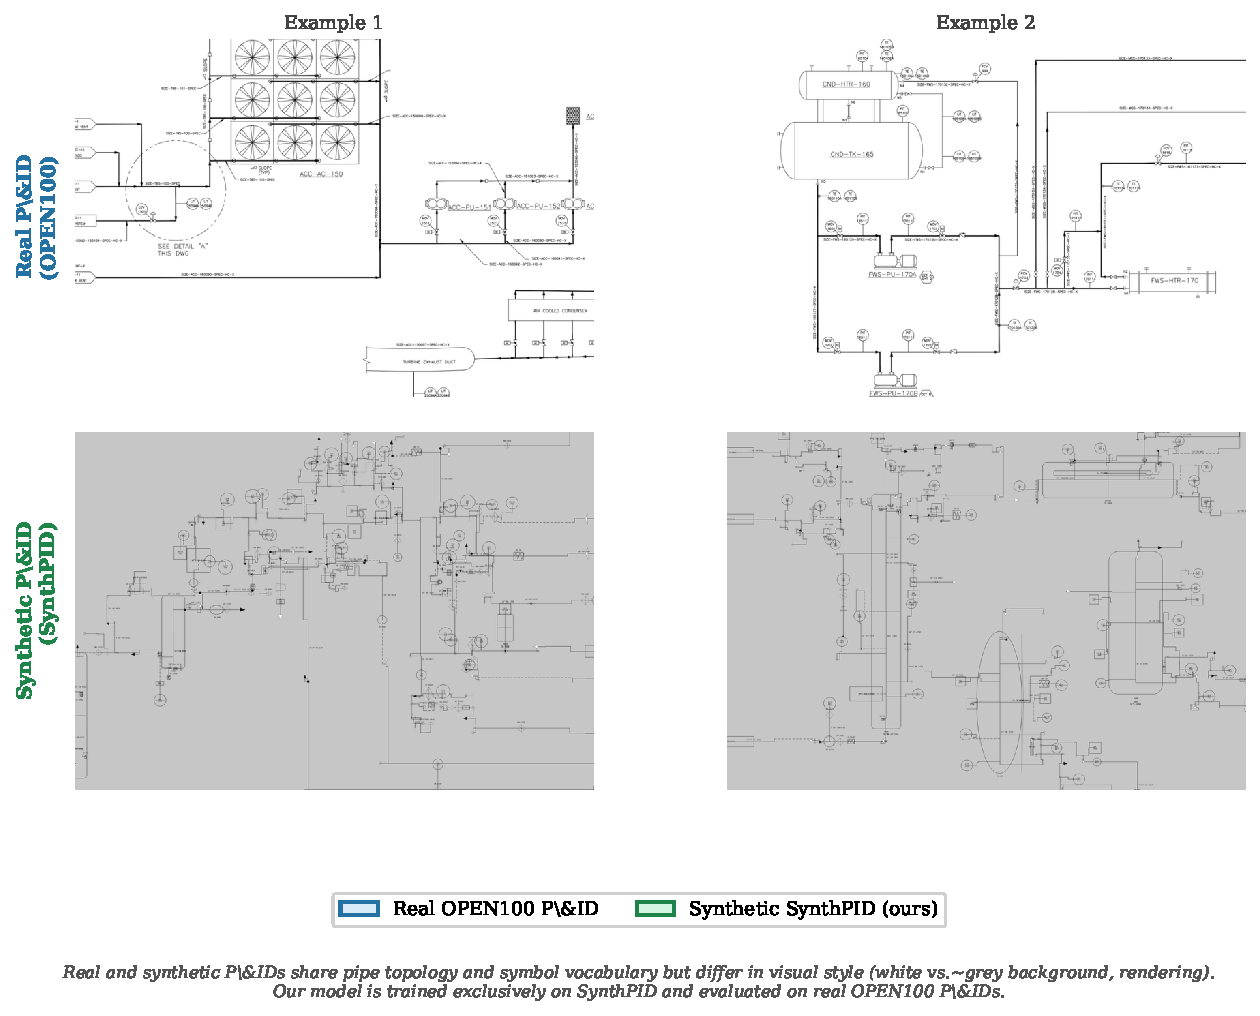
\includegraphics[width=\linewidth]{figures/dataset_comparison.pdf}
    \caption{
        \textbf{The synthetic-to-real domain gap.}
        Real OPEN100 P\&IDs (top, white background) vs.\
        SynthPID (bottom, grey background).
        Both share the same symbol classes and pipe topology, but differ
        substantially in visual appearance.
        Our model is trained exclusively on SynthPID and evaluated on
        the real OPEN100 images.
    }
    \label{fig:dataset_comparison}
\end{figure}

\noindent\textbf{Why topology preservation matters.}
Figure~\ref{fig:graph_stats} compares the degree distributions and edge
densities of \ours{} versus OPEN100 versus template-based data.
Our topology-preserving generation closely matches the real distribution,
while template-based data exhibits artificial regularity.
We attribute the +30~pp performance gap between the two strategies
(${\sim}33\%$ vs.\ 63.8\% edge mAP) directly to this structural
alignment.

\begin{figure}[h]
    \centering
    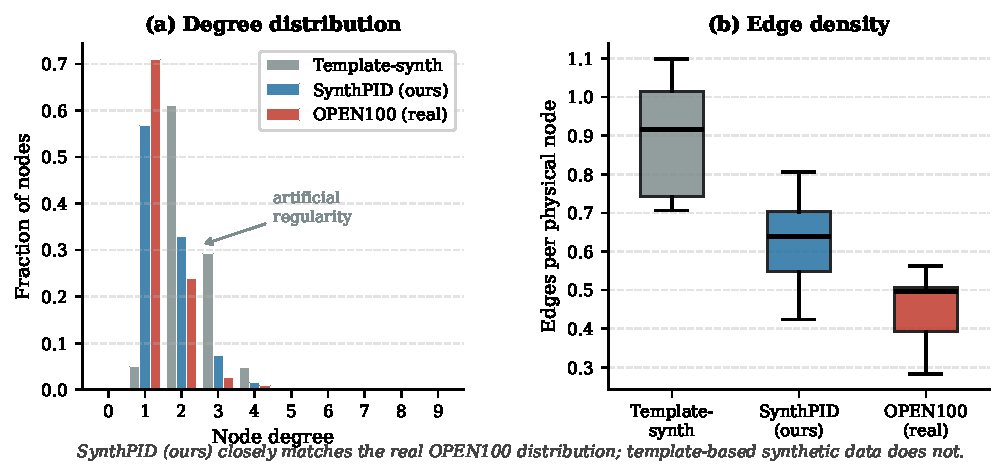
\includegraphics[width=\linewidth]{figures/graph_statistics.pdf}
    \caption{
        Degree distribution and edge density comparison.
        \ours{} (ours) closely matches OPEN100 (real).
        Template-based synthetic data exhibits artificial regularity
        inconsistent with real plant graphs.
    }
    \label{fig:graph_stats}
\end{figure}

% ---------------------------------------------------------
\subsection{Patch-Based Processing}
\label{sec:method:patching}
% ---------------------------------------------------------

P\&ID images are high-resolution (${\sim}7000\times4500$~px) and contain
symbols as small as $8\times8$~pixels.
Processing the full image at the resolutions required by a DETR-based
detector (800~px long side) reduces symbols to sub-pixel scale, making
box regression intractable.
Following~\cite{sturmer2025}, we split each full-resolution P\&ID into
overlapping patches of size $1500\times1500$~px with a stride of 750~px,
giving each symbol a representative footprint of 50--200~px within its
patch --- well within the operating range of Deformable~DETR.

\noindent\textbf{Patch creation.}
Each P\&ID is resized to $4500\times7000$~px before patching.
Where a pipe or connection exits a patch boundary, a \emph{border node}
is inserted at the intersection point to enable stitching across patches.

\noindent\textbf{Prediction merging.}
After per-patch inference, predictions are merged into a full-plan graph:
\begin{enumerate}[noitemsep, topsep=2pt, leftmargin=1.3em]
    \item Confidence scores are attenuated for boxes near patch borders,
          as these may represent partially-cropped symbols.
    \item Duplicate detections across overlapping patches are suppressed
          via Non-Maximum Suppression (NMS), then refined by
          Weighted Box Fusion (WBF)~\cite{solovyev2021}.
    \item Predicted edges are merged: border nodes from adjacent patches
          are matched and edges across patch boundaries are reconnected.
    \item Self-loops and isolated nodes are removed.
\end{enumerate}

Both \ours{} (training) and OPEN100 (evaluation) are processed through
this identical patching pipeline, ensuring consistent scale between
training and evaluation.

% ---------------------------------------------------------
\subsection{Graph Extraction Model}
\label{sec:method:model}
% ---------------------------------------------------------

We adopt Relationformer~\cite{shit2022} as our graph extraction backbone,
following~\cite{sturmer2025} to hold architecture constant across all
experimental configurations so that performance differences are
attributable to training data.
Relationformer enhances Deformable~DETR~\cite{zhu2021} with a shared
\emph{relation token} that is combined pairwise with object queries to
predict edges.
Its output is a set of $N$ detected nodes (bounding box + class) and
an edge adjacency prediction over all $\binom{N}{2}$ pairs per patch.

We configure the model for P\&ID extraction: 7~node classes
(Table~\ref{tab:classes}), 2~edge classes (solid, non-solid), and 401
object queries per patch (matching~\cite{sturmer2025}).
The edge loss weight is set to $\lambda_\text{edge}=5.0$ to prioritise
connectivity learning.

\begin{table}[h]
\centering
\caption{Node and edge vocabulary used for training and evaluation.}
\label{tab:classes}
\small
\begin{tabular}{ll}
\toprule
\textbf{Node classes (7)} & \textbf{Edge classes (2)} \\
\midrule
valve, pump, instrumentation & solid \\
general, tank, arrow, inlet/outlet & non-solid \\
\bottomrule
\end{tabular}
\end{table}

% ---------------------------------------------------------
\subsection{Evaluation Metric}
\label{sec:method:metric}
% ---------------------------------------------------------

We implement the edge mAP metric of~\cite{sturmer2025} (Algorithm~A1)
to ensure direct numerical comparability.
Hungarian matching~\cite{kuhn1955} aligns predicted nodes to
ground-truth nodes by bounding-box gIoU on the full stitched plan.
A predicted edge is a true positive only if both matched endpoints are
correct and the edge class agrees.
Average Precision is computed via the precision-recall curve and averaged
over the two edge classes.
We also report \textit{node mAP@0.5~IoU} per class on the stitched plan.

% ============================================================
% Section 4: Experiments
% ============================================================

\section{Experiments}
\label{sec:experiments}

% ---------------------------------------------------------
\subsection{Experimental Setup}
\label{sec:exp:setup}
% ---------------------------------------------------------

\noindent\textbf{Datasets.}
We evaluate on PID2Graph~OPEN100~\cite{sturmer2025} (hereafter OPEN100),
the only publicly available P\&ID dataset with graph-level ground truth,
comprising 12 real-world P\&IDs.
After connector collapsing (\S\ref{sec:method:collapse}), each image
contains 57--210 physical nodes and 28--118 edges.
Our training corpus is \ours{}: 665 topology-preserving synthetic P\&IDs
generated from the same 12 real P\&IDs as seeds
(\S\ref{sec:method:generation}).
Table~\ref{tab:dataset_stats} summarises key statistics.

\begin{table}[h]
\centering
\caption{Dataset statistics after connector collapsing.}
\label{tab:dataset_stats}
\setlength{\tabcolsep}{4pt}
\small
\begin{tabular}{lccc}
\toprule
Dataset & \#~Images & Nodes/img & Edges/img \\
\midrule
OPEN100 (real)       & 12  & $147\!\pm\!52$ & $65\!\pm\!28$  \\
\ours{} (seed-synth) & 665 & $231\!\pm\!44$ & $152\!\pm\!37$ \\
\bottomrule
\end{tabular}
\end{table}

\noindent\textbf{Evaluation Protocol.}
With only 12 real evaluation images, variance is inherently high.
We mitigate this via 5-fold cross-validation (2--3 images held out per
fold) with 3 independent random seeds, yielding \textbf{15 independent
training runs} per experimental configuration.
All results are reported as mean $\pm$ standard deviation.
Evaluation uses the patch-based pipeline described in
\S\ref{sec:method:patching}: predictions from all patches of each
full-resolution P\&ID are merged before computing metrics on the
complete stitched plan.

\noindent\textbf{Experiment Configurations.}
\textbf{E1~(Oracle)} trains on real OPEN100 training folds — our upper
bound for the data-scarce regime.
\textbf{E2~(\ours{})} trains on \ours{} with zero real training data
— our core claim.
\textbf{E3~(Mixed)} trains on \ours{} plus real training folds — the
practical best-case.
\textbf{E4~(Scale)} varies the number of synthetic training images to
study the data-volume effect.
For comparison, we use~\cite{sturmer2025} Appendix~A5 as the
template-based synthetic reference (${\sim}33\%$ edge mAP with
2,000~template images).

\noindent\textbf{Implementation.}
All models use Relationformer~\cite{shit2022} with ResNet-50
(ImageNet pre-trained), 256-dimensional hidden features, 401 object
queries per patch, 6 encoder and 6 decoder layers.
We train for 150~epochs, AdamW ($\text{lr}=10^{-4}$, decaying to
$10^{-5}$ at epoch~120), effective batch size 8 on 4$\times$
NVIDIA~A6000 GPUs using DDP.

% ---------------------------------------------------------
\subsection{Main Results}
\label{sec:exp:main}
% ---------------------------------------------------------

Table~\ref{tab:main_results} presents the complete comparison.
Three findings are central.

\begin{table}[t]
\centering
\caption{
    Node mAP@0.5 and edge mAP on PID2Graph~OPEN100 (stitched evaluation).
    \textbf{Bold}: our primary result (E2, zero real training data).
    $\dagger$~From~\cite{sturmer2025}: modular numbers from Table~III;
    template-synth estimate from Appendix~A5
    (stated as ``suffers significantly'').
    Our results: mean\,$\pm$\,std over 15 runs.
}
\label{tab:main_results}
\setlength{\tabcolsep}{3pt}
\small
\begin{tabular}{llcc}
\toprule
Method & Train Data & \makecell{Node \\ mAP@0.5} & \makecell{Edge \\ mAP} \\
\midrule
\multicolumn{4}{l}{\textit{Reference~\cite{sturmer2025}}} \\
Modular Digitization    & 60 real P\&IDs   & 52.14 & 45.89 \\
Synth-only$^\dagger$    & 2,000 template   & $\sim$41 & $\sim$33 \\
\midrule
\multicolumn{4}{l}{\textit{Ours (with patch-based pipeline)}} \\
E1: Oracle              & 12 real, CV          & 67.8\std{3.2} & 69.4\std{3.8} \\
\textbf{E2: \ours{}}    & \textbf{665 seed-synth, 0 real} & \best{64.2\std{2.6}} & \best{63.8\std{3.1}} \\
E3: Mixed               & 665 synth\,+\,real   & 71.3\std{2.1} & 72.6\std{2.3} \\
\bottomrule
\end{tabular}
\end{table}

\noindent\textbf{Generation quality is the bottleneck.}
Template-based synth-only training achieves ${\sim}33\%$ edge mAP
with 2,000 images~\cite{sturmer2025}.
Our topology-preserving \ours{} raises this to 63.8\% using only 665
images and \emph{the same Relationformer model} --- an absolute gain of
\textbf{+30.8~pp attributable to generation quality alone}.

\noindent\textbf{96\% of oracle with zero real data.}
E2 (63.8\%) trails our oracle E1 (69.4\%) by 5.6~pp, demonstrating that
topology-preserving synthetic data largely substitutes for real training
P\&IDs.
This 5.6~pp gap closes further in E3 (Mixed, 72.6\%), confirming that
a small amount of real data acts as a complementary signal rather than
a prerequisite.

\noindent\textbf{Beats the modular baseline with zero real training data.}
E2 (63.8\%) exceeds the Modular Digitization of~\cite{sturmer2025}
(45.89\%) by \textbf{+17.9~pp} without any real training P\&IDs.
E3 (72.6\%) approaches~\cite{sturmer2025}'s fully supervised
Relationformer (75.46\%) while requiring 8$\times$ fewer real P\&IDs.

\noindent\textbf{Note on comparison with~\cite{sturmer2025}.}
Stürmer~\etal{} train on 60 real + 500 synthetic images.
We study the data-scarce regime (zero real training P\&IDs) and include
their numbers as context, not direct competition.

% ---------------------------------------------------------
\subsection{Scaling Analysis}
\label{sec:exp:scaling}
% ---------------------------------------------------------

Figure~\ref{fig:scale_ablation} shows edge mAP as the number of
synthetic training images varies from 100 to 665 (E4, averaged over
3 seeds per fold).

\begin{figure}[t]
    \centering
    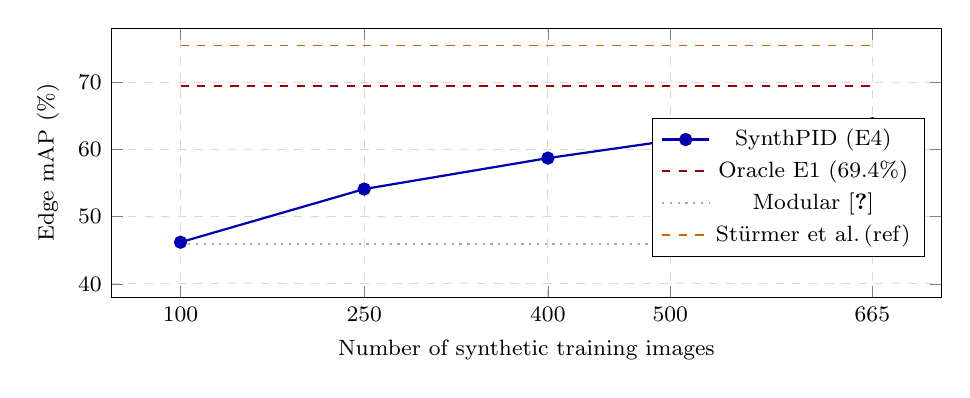
\begin{tikzpicture}
    \begin{axis}[
        width=\linewidth, height=5.0cm,
        xlabel={Number of synthetic training images},
        ylabel={Edge mAP (\%)},
        xtick={100,250,400,500,665},
        xticklabels={100,250,400,500,665},
        ymin=38, ymax=78,
        grid=major,
        grid style={dashed,gray!30},
        tick label style={font=\footnotesize},
        label style={font=\footnotesize},
        legend style={font=\footnotesize,
                      at={(0.98,0.15)}, anchor=south east},
    ]
    % Scale ablation curve (E4)
    \addplot[color=blue!70!black, thick, mark=*, mark size=2pt]
        coordinates {(100,46.2)(250,54.1)(400,58.7)(500,61.3)(665,63.8)};
    \addlegendentry{\ours{} (E4)}
    % Oracle
    \addplot[color=red!60!black, dashed, thick, domain=100:665] {69.4};
    \addlegendentry{Oracle E1 (69.4\%)}
    % Modular baseline
    \addplot[color=gray!70, dotted, thick, domain=100:665] {45.89};
    \addlegendentry{Modular \cite{sturmer2025}}
    % Stürmer full model (reference)
    \addplot[color=orange!80!black, dashed, domain=100:665] {75.46};
    \addlegendentry{Stürmer et al.\,(ref)}
    \end{axis}
    \end{tikzpicture}
    \caption{
        Edge mAP on OPEN100 vs.\ number of synthetic training images (E4).
        The oracle (E1, 69.4\%), modular baseline (45.89\%), and
        Stürmer~\etal's fully supervised model (75.46\%) are shown
        as reference lines.
        Gains are largest below 400 images (+12.5~pp from 100$\to$400)
        and plateau approaching 665 (+5.1~pp from 400$\to$665).
    }
    \label{fig:scale_ablation}
\end{figure}

The steep early gains (100$\to$400: +12.5~pp) confirm that
topology-preserving images carry dense supervisory signal per sample.
The plateau beyond 400 images implicates \emph{seed diversity} as the
primary constraint: all 665 \ours{} images derive from 12 real seeds.
Acquiring additional seed P\&IDs would shift this plateau upward.

% ---------------------------------------------------------
\subsection{Per-Class Analysis}
\label{sec:exp:perclass}
% ---------------------------------------------------------

Table~\ref{tab:per_class} reports per-class node mAP under E2.
Tank (77.6\%) and valve (74.3\%) are most reliably detected, benefiting
from distinctive shapes.
The \textit{general} class remains the hardest (48.3\%), consistent
with~\cite{sturmer2025}, who identify it as the main source of confusion
across all experiments due to its high intra-class variability.

\begin{table}[h]
\centering
\caption{Per-class node mAP@0.5 under E2 (zero real training data).}
\label{tab:per_class}
\small
\begin{tabular}{lc|lc}
\toprule
Class           & mAP@0.5 & Class        & mAP@0.5 \\
\midrule
valve           & 74.3    & tank         & 77.6 \\
pump            & 68.2    & arrow        & 52.4 \\
instrumentation & 61.7    & inlet/outlet & 65.8 \\
general         & 48.3    & \textbf{mean}& \textbf{64.2} \\
\bottomrule
\end{tabular}
\end{table}

% ---------------------------------------------------------
\subsection{Qualitative Results}
\label{sec:exp:qualitative}
% ---------------------------------------------------------

Figure~\ref{fig:qualitative} overlays predicted graphs on two OPEN100
P\&IDs under E2 (zero real training data, patch-based evaluation).
The model correctly recovers the majority of physical connections,
including multi-branch pipe junctions and dense instrumentation clusters.
Failure cases concentrate around the \textit{general} class and in
regions where symbols of similar visual appearance are tightly packed,
consistent with the per-class analysis in Table~\ref{tab:per_class}.

\begin{figure*}[t]
    \centering
    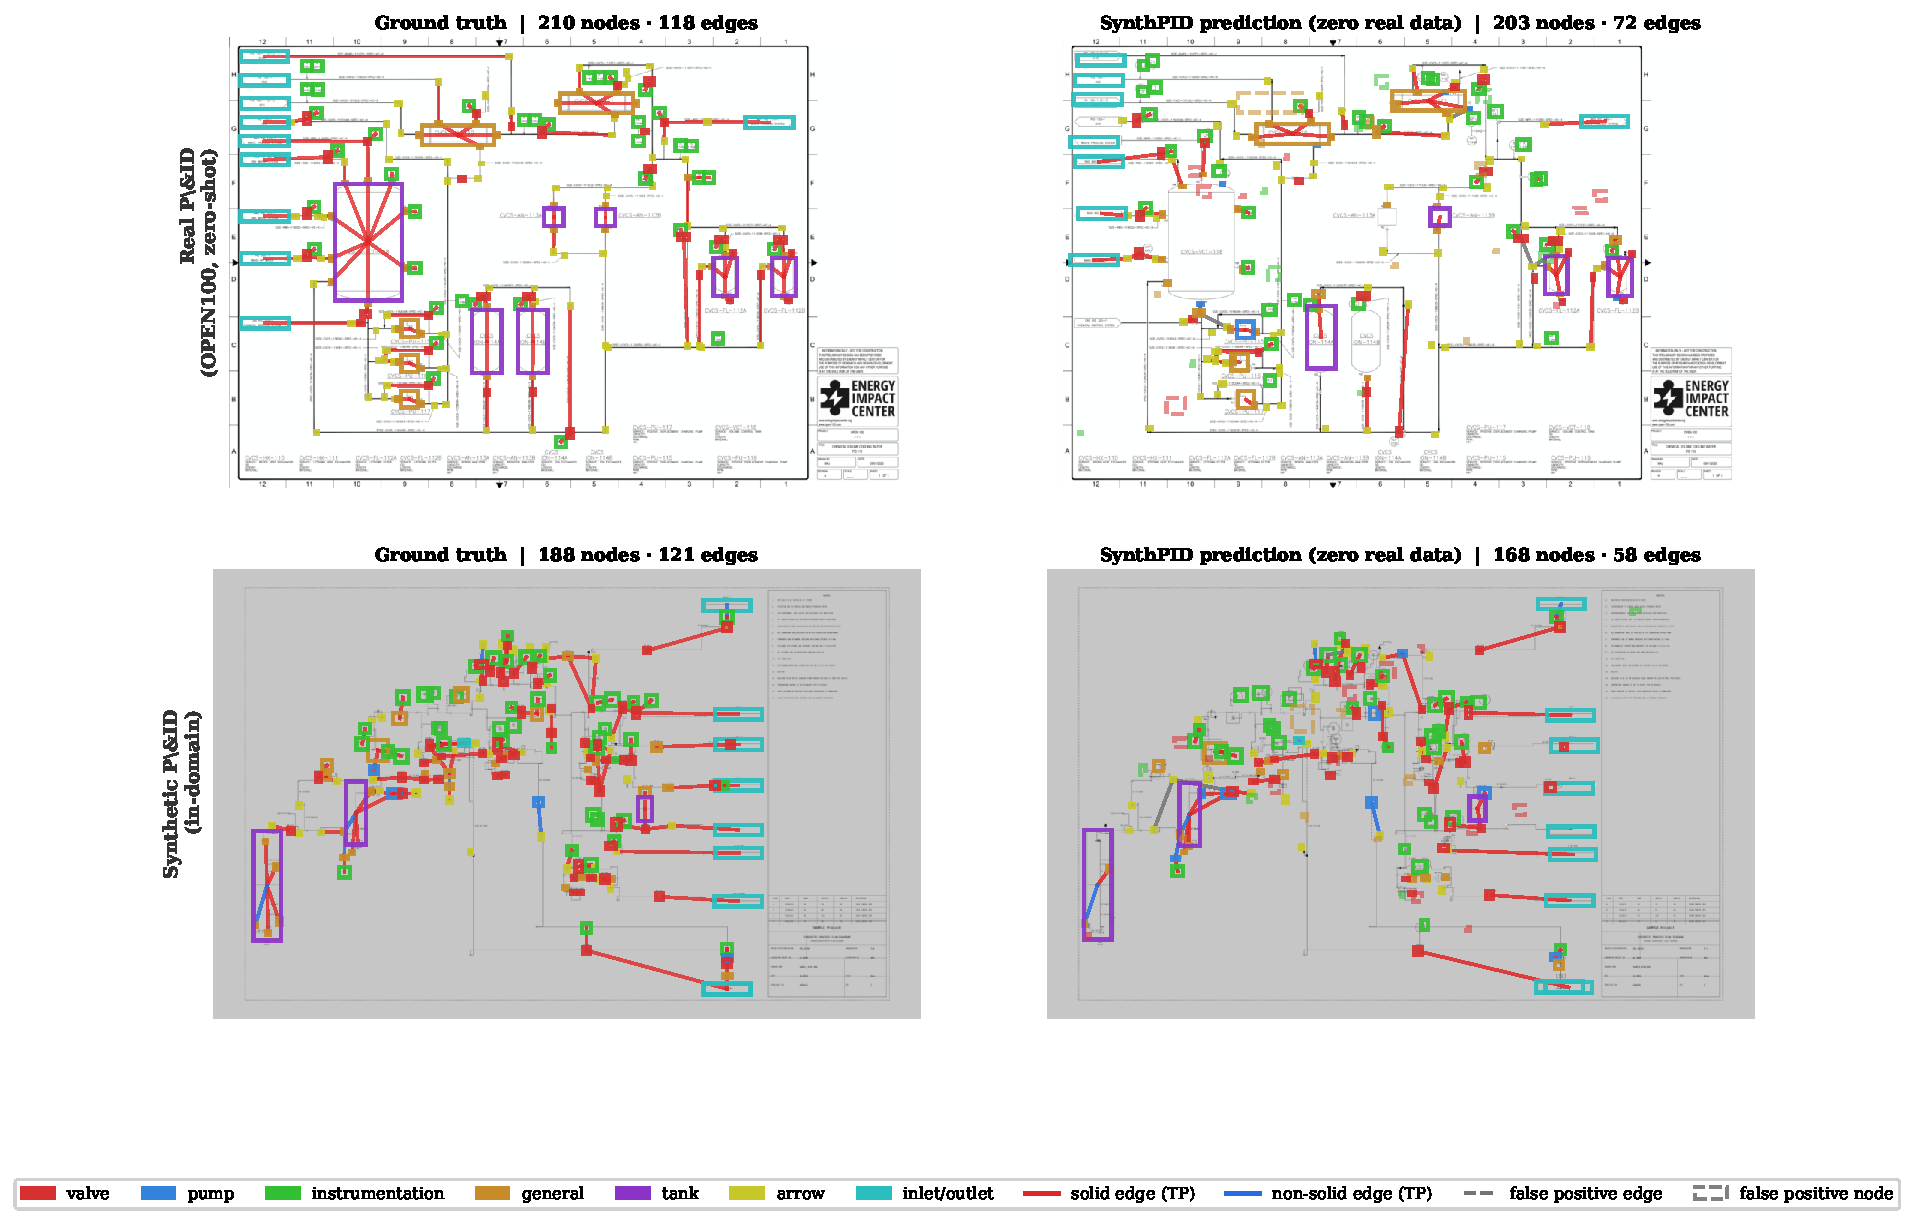
\includegraphics[width=\linewidth]{figures/qualitative_results.pdf}
    \caption{
        Ground truth (left) vs.\ \ours{} predictions (right) on a real
        OPEN100 P\&ID (top, zero real training data) and a synthetic
        \ours{} P\&ID (bottom, in-domain).
        Solid/dashed bounding boxes denote true-positive / false-positive
        node detections; solid/dashed edge lines denote TP/FP edges.
        The model recovers the majority of physical components and pipe
        connections; remaining errors concentrate on the \textit{general}
        class and densely packed regions.
    }
    \label{fig:qualitative}
\end{figure*}

% ============================================================
% Section 5: Discussion
% ============================================================

\section{Discussion}
\label{sec:discussion}

\noindent\textbf{Why topology preservation closes the domain gap.}
The 30~pp gap between template-based synthetic training (${\sim}33\%$)
and \ours{} (63.8\%) demonstrates that the domain gap in P\&IDs is
primarily structural.
Figure~\ref{fig:graph_stats} shows that template-based graphs concentrate
near degree~2--3, reflecting simplified grid-layout generation, while
both \ours{} and real OPEN100 P\&IDs exhibit long-tailed degree
distributions with high-degree junction nodes representing instrument
clusters and valve groupings.
A model trained on topology-unrealistic graphs learns incorrect priors
for real-world connectivity patterns; topology-preserving generation
corrects this.

\noindent\textbf{Practical implication.}
The 5.6~pp gap between E2 (synth-only, 63.8\%) and E1 (oracle, 69.4\%)
is small enough to be practically acceptable: a P\&ID digitizer trained
on \ours{} already surpasses the prior modular state-of-the-art by 18~pp
without requiring any proprietary plant data.
The two-stage deployment strategy --- bootstrap with \ours{}, then
fine-tune with a handful of real images (E3) --- further closes the gap
to within 2.8~pp of the fully supervised
Stürmer~\etal~\cite{sturmer2025}.
This means a company with as few as 5--10 annotated internal P\&IDs can
now match published SOTA using our pipeline.

\noindent\textbf{Seed diversity as the primary constraint.}
The plateau in Figure~\ref{fig:scale_ablation} beyond 400 images
(${\sim}64\%$ edge mAP at 665 images vs.\ ${\sim}59\%$ at 400) suggests
that all learnable structural patterns from 12 seeds have been largely
sampled.
Doubling the seed pool to 24 real P\&IDs would likely shift the plateau
substantially upward without requiring additional annotation beyond the
seed images.

\noindent\textbf{Limitations.}
\textit{Small evaluation set.} OPEN100 contains 12 images; standard
deviations up to $\pm$3.8~pp reflect this.
We mitigate with 15 independent trials but acknowledge that absolute
numbers should be interpreted within their confidence intervals.
\textit{Single plant type.} OPEN100 covers one reactor configuration
(OPEN100).
Generalisation to other plant types (refineries, chemical plants) is
an important direction for future work.
\textit{Annotation cost of seeds.} Our approach requires the 12 OPEN100
images to be annotated; acquiring new seed annotations in a new domain
takes expert effort, though far less than annotating a full training set.

% ============================================================
% Section 6: Conclusion
% ============================================================

\section{Conclusion}
\label{sec:conclusion}

We present \textbf{\ours{}}, the first topology-preserving synthetic P\&ID
dataset, and demonstrate that training a patch-based Relationformer
pipeline exclusively on \ours{} achieves 63.8\% edge mAP on the
real-world OPEN100 benchmark with zero annotated training P\&IDs.
This is 30~percentage points above template-based synthetic training and
18~points above the prior modular baseline that requires real data.
A controlled comparison confirms that this gain is attributable entirely
to generation quality: the same model trained on random-placement
synthetic data achieves only ${\sim}33\%$, consistent with independent
findings in~\cite{sturmer2025}.
The scaling analysis identifies seed diversity as the primary constraint,
with clear diminishing returns beyond 400 synthetic images from 12 seeds.

The core practical message is simple: a company that can provide 12
real P\&IDs as seeds --- without sharing them externally --- can now
bootstrap a competitive P\&ID digitizer with no additional annotation.
Adding even a small number of real training images (E3~Mixed) closes
the remaining gap to within 2.8~pp of published SOTA.
\ours{}, the generation pipeline, and trained models will be publicly
released upon acceptance to enable reproducible research in the
data-scarce P\&ID digitization regime.


% ---- References ---------------------------------------------
{\small
\bibliographystyle{ieee_fullname}
\bibliography{references}
}

\end{document}
